\chapter[Background and Related Work]{\texorpdfstring{Background and\\Related Work}{Background and Related Work}}
\label{chap:related}

\section{Cloud GPU Computing}
\label{sec:cloud-gpu-computing}

General-purpose computation on graphics hardware became practical with NVIDIA's CUDA platform~\cite{nickolls2008scalable}, and GPU computing was subsequently offered as a cloud service. Early cloud providers (AWS, Azure, GCP) offered GPU instances as part of virtual machine (VM) rental services, billed hourly with a minimum session length of a full hour on AWS~\cite{barr2017persecond}. The rise of deep learning as a primary GPU workload in the 2010s drove rapid expansion of GPU instance types and the emergence of spot-pricing markets where unused capacity is offered at discounted rates with potential preemption~\cite{yi2010reducing,subramanya2015spoton,zheng2015bid}.

By the early 2020s, a second tier of GPU cloud providers, such as RunPod, Lambda, CoreWeave, and Vast.ai, had emerged, some with billing granularity as fine as one second~\cite{runpod2026podspricing,vastai2026concepts}. Marketplace-style platforms such as RunPod and Vast.ai aggregate GPU hardware from data-centre operators and individual hosts~\cite{runpod2026podsoverview,vastai2026concepts}, and these providers collectively offer a heterogeneous catalogue of GPU types~\cite{runpod2026podspricing,coreweave2026pricing,lambda2026pricing} (consumer-grade RTX series, workstation-grade A-series, data-centre A100/H100) at widely varying price points. For rendering workloads, which tend to be short (tens of seconds to a few minutes per frame) and embarrassingly parallel at the frame level, per-second billing and the ability to spin up many low-cost nodes simultaneously make these platforms attractive alternatives to dedicated render farms.

The key distinguishing feature of on-demand cloud GPU rental relevant to this thesis is \emph{qualitative availability}. Unlike reserved VM instances with guaranteed exclusive access and pre-provisioned capacity, an on-demand instance must be acquired afresh from a pool whose stock fluctuates with competing demand: when stock is scarce, acquiring an instance of a given type incurs a provisioning delay. From the perspective of the scheduling algorithm, this manifests as a coarsened observable state: the platform API exposes a qualitative per-type stock status, but not the underlying cause (customer demand, maintenance, hardware fault). This is the abstraction encoded in the CGRSP stochastic availability model, which targets the RunPod Secure Cloud on-demand model (where a running instance is not reclaimed) rather than spot preemption.

A critical distinction separating marketplace GPU rental from the managed-cluster context of most scheduling literature is rarely made explicit. \textbf{Reserved-cluster schedulers}, including HEFT~\cite{topcuoglu2002heft}, Gavel~\cite{narayanan2020gavel}, and Optimus~\cite{peng2018optimus}, operate on machine or GPU pools under the operator's exclusive control; node availability is guaranteed and the scheduling problem reduces to job-to-node assignment. \textbf{Marketplace scheduling}, by contrast, must treat GPU availability as externally determined: competing customer demand, platform maintenance windows, and hardware failures collectively determine which GPU types can be provisioned at any given moment, outside the operator's control. This distinction is structural, not incidental: the scheduler must treat availability as a stochastic first-class input rather than a deterministic constraint. This is precisely the gap the CGRSP formulation closes. A third body of work, \textbf{spot and transient-instance scheduling}, does treat cloud availability as stochastic, but models it as mid-job \emph{revocation} risk: checkpointing against instance loss~\cite{yi2010reducing}, batch services that absorb revocations~\cite{subramanya2015spoton}, and bidding strategies over spot price processes~\cite{zheng2015bid}. The on-demand Secure Cloud setting of this thesis is structurally different: a held instance is never reclaimed, so no checkpoint or migration machinery is relevant, and scarcity manifests instead as a stochastic provisioning delay at acquisition time, observed only as a coarse per-type stock status inside every dispatch decision. That acquisition-side availability problem is the one the surveyed spot literature does not address.

Recent work has moved closer to the marketplace setting without reaching it. SkyNomad~\cite{li2026skynomad} schedules deadline-bound GPU batch jobs across spot instances in several cloud regions, probing whether spot capacity can currently be obtained in each region and predicting how long an instance will survive before preemption, but it treats availability as a binary per-region signal backed by an always-available on-demand fallback, makes decisions for a single job rather than dispatching a queue of jobs, and treats the deadline as a hard guarantee under a cost-minimising objective. REACH~\cite{yu2025reach} targets community GPU platforms that aggregate peer-contributed consumer GPUs, the topology closest to a GPU marketplace, but it models the volatile reliability of nodes during execution with a learned transformer-based policy rather than scarcity at acquisition time. BOA Constrictor~\cite{li2026boa} takes the renter's side of cloud GPU rental, deciding how many GPUs of each priced type to rent under a long-run budget, yet it assumes rented capacity is always obtainable and optimises mean job completion time with no deadlines. None of the three observes availability as a coarse stock status at dispatch time, which is the setting CGRSP formalises.

\section{Classical Job Scheduling}
\label{sec:classical-job-scheduling}

Job scheduling on a set of machines to minimise one or more performance criteria is one of the most well-studied topics in operations research and computer science~\cite{pinedo2016scheduling}. Graham et al.~\cite{graham1979optimization} established the three-field notation $\alpha|\beta|\gamma$ for scheduling problems. For CGRSP, the problem is closest to $P_m|\text{online}, r_j, d_j|\sum \omega_j C_j$ (parallel identical machines with online arrivals, release times, deadlines, and weighted completion time; the weight is written $\omega_j$ here to avoid a clash with the waiting time $w_j$), except that the machines in CGRSP are not identical: they differ in speed and cost, and their speed ranking depends on the job, making it a generalisation to unrelated parallel machines ($R_m$) rather than uniform parallel machines ($Q_m$). A uniform-machine model would require one speed factor per machine that applies to every job, and the fleet violates this, because the stratum means rank the types differently across complexity levels: at $\kappa=1$ the RTX~3090 (59.5\,s) edges the RTX~A5000 (60.7\,s), at $\kappa=2$ the A5000 (69.1\,s) edges the 3090 (69.6\,s), and at $\kappa=3$ the RTX~A4500 is fastest (88.3\,s), followed by the 3090 (91.2\,s), the A5000 (94.5\,s) and the A4000 (98.6\,s) (Table~\ref{tab:gpu_specs}). The $\kappa=1$ cells for the A4000 and A4500, and the sparse $\kappa=2$ A4000 cell, are model estimates rather than measurements (Section~\ref{sec:gpu-fleet-model}), and these are observational stratum means rather than scene-matched comparisons, so the ranking is a property of the workload mix as much as of the hardware.

\subsection{Shortest Processing Time (SPT)}
\label{ssec:shortest-processing-time-spt}

The Shortest Processing Time rule assigns the available processor to the ready job with the smallest processing time. Smith~\cite{smith1956various} proved that ordering jobs by processing time divided by weight (WSPT) minimises total weighted completion time on a single machine; with equal weights this reduces to SPT, which therefore minimises average completion time. On identical parallel machines, SPT list scheduling (assigning the shortest unscheduled job to whichever machine becomes free next) remains optimal for minimising total completion time, and hence average flow time, in the offline setting with all jobs available at time zero~\cite{pinedo2016scheduling}. In online settings with Poisson arrivals, SPT minimises mean response time among non-preemptive policies (a classical result from M/G/1 queueing theory~\cite{pinedo2016scheduling}). SPT's weakness in deadline-constrained settings is its tendency to starve large, long-running jobs: a steady stream of short jobs keeps a machine busy and can delay deadline-critical long jobs past their deadlines.

\subsection{Earliest Deadline First (EDF)}
\label{ssec:earliest-deadline-first-edf}

Earliest Deadline First, attributed to Jackson~\cite{jackson1955scheduling}, whose deadline ordering Lawler and Moore~\cite{lawler1969functional} later built into an exact dynamic-programming method for the weighted number of tardy jobs, prioritises the ready job with the nearest deadline. EDF is optimal on a single preemptive machine in the feasibility sense: if any policy can meet every deadline, EDF does~\cite{dertouzos1974control}; Liu and Layland~\cite{liu1973scheduling} established the corresponding 100\% utilisation bound for periodic task sets. On non-preemptive parallel machines, the setting of CGRSP, EDF does not provide a worst-case guarantee for deadline violation minimisation. The Phase~3 deadline sensitivity experiments in Chapter~\ref{chap:experiments} instead separate its comparison against shortest-job-first ordering (SPT) into three regimes: EDF attains significantly lower miss when the tight-deadline fraction is low ($\leq 30\%$; at $30\%$, $t=\DlThirtySPTEDFmissT$, $\DlThirtySPTEDFmissP$), the paired test does not resolve their difference at the midpoint of the sweep ($50\%$, $t=\DlFiftySPTEDFmissT$, $\DlFiftySPTEDFmissP$), and SPT attains significantly lower miss at high tight fractions ($\geq 70\%$; at $70\%$, $t=\DlSeventySPTEDFmissT$, $\DlSeventySPTEDFmissP$).

\subsection{First-In-First-Out (FIFO)}
\label{ssec:first-in-first-out-fifo}

FIFO processes jobs in the order they arrive. It provides fairness guarantees (no starvation), requires no knowledge of processing time or deadline, and has long served as the default scheduling policy in batch computing systems, dating to the earliest resident-monitor mainframe operating systems~\cite{silberschatz2018operating}. FIFO is used as the primary baseline in this study because it represents the ``do nothing special'' approach. In the M/M/c queueing model, FIFO achieves the same throughput as any work-conserving policy (by work-conservation arguments~\cite{pinedo2016scheduling}), but it does not minimise mean response time or deadline adherence.

\subsection{Other Heuristics}
\label{ssec:other-heuristics}

\textbf{Lowest Cost First (LCF)} prioritises the GPU type with the lowest effective rental cost per job, defined as the product of the rental rate and the expected execution time: $\text{cost}_{\text{eff}}(j, m) = p_{g(m)} \cdot \mathbb{E}[W(\kappa_j, g(m))]$. LCF is motivated by cost-minimisation objectives, relevant for rendering studios operating under tight production budgets where deadline pressure is low. A complicating factor is GPU availability reliability: a ``cheap'' GPU type with consistently low stock may increase effective turnaround through long provisioning delays. This is addressed in the CGRSP implementation through a proportional stock-status penalty added to the effective cost.

\textbf{Balanced scheduling} combines processing speed (SPT-like) and cost (LCF-like) criteria through a weighted composite score. A weight $w_b \in [0, 1]$ controls the trade-off: $w_b \to 1$ approaches SPT behaviour (speed priority), $w_b \to 0$ approaches LCF (cost priority). In the CGRSP implementation, $w_b = 0.8$ (speed-biased) is used, with global-max normalisation to prevent one criterion from dominating due to differing numerical scales. (The weight is written $w_b$ to avoid a clash with the objective weights $\alpha_1, \alpha_2$ of Chapter~\ref{chap:formulation}.) Unlike EDF and SPT, Balanced does not reorder jobs; it sorts only on node selection, maintaining FIFO job ordering. This design choice ensures that Balanced is statistically distinguishable from both EDF (which reorders by deadline) and SPT (which reorders by processing time) in the comparative evaluation.

\section{Heterogeneous Machine Scheduling}
\label{sec:heterogeneous-machine-scheduling}

When machines have different speeds, the scheduling problem becomes significantly harder. Braun et al.~\cite{braun2001comparison} provided the first systematic comparison of scheduling heuristics on heterogeneous machines, evaluating 11 algorithms including min-min, max-min, genetic algorithms, and simulated annealing in terms of makespan. Their study on synthetic workloads found that the relatively simple min-min heuristic, which repeatedly selects, among all unmapped tasks, the one with the smallest earliest-completion time and assigns it to that machine, performs well in comparison with far more complex search methods, although the genetic algorithm produced the best mappings overall. CGRSP's SPT policy (Chapter~\ref{chap:system}) resembles a single-pass form of min-min restricted to the currently idle nodes: at each scheduling event it orders the queued jobs by their best expected execution time over the idle nodes, which equals the earliest completion time min-min selects on only when the stock-dependent provisioning delay that every CGRSP dispatch incurs (Chapter~\ref{chap:formulation}) is set aside or stock is uniform across the idle nodes; it also computes that ordering once per event rather than after every assignment. It then places each job using a composite of speed, cost, and stock status, which reduces to the minimum-completion-time (MCT) machine choice of the same study only when cost and stock are uniform across the idle nodes.

The Heterogeneous Earliest Finish Time (HEFT) algorithm of Topcuoglu et al.~\cite{topcuoglu2002heft} is the most widely cited heuristic for scheduling task-dependency DAGs on heterogeneous parallel machines. HEFT ranks tasks by upward rank (estimated time to completion including successors) and assigns each task to the machine that minimises its finish time. For CGRSP, jobs are independent (no DAG dependencies), so each job's upward rank collapses to its mean execution time across machine types, and HEFT reduces to longest-average-job-first ordering with earliest-finish-time machine selection. It therefore orders jobs in the reverse of the SPT policy described in Chapter~\ref{chap:system}, and, unlike HEFT, SPT selects nodes by a composite of speed, cost, and stock status rather than by earliest finish time alone.

GPU program schedulers operate at a finer granularity. Chien et al.~\cite{chien2018graph} represent an OpenCL program as a computational graph of kernels with their metadata and dependencies, then schedule kernel tasks across heterogeneous CPU and GPU devices, using code analysis to choose the target device and work-group size. Chang et al.~\cite{chang2020dependent} develop a framework for dependent GPU programs, where kernel ordering is considered together with memory write-back policy to avoid unnecessary data movement. Both operate within a single node and optimise execution performance; the decisions are kernel order, device choice and memory policy, not which rented node receives which job. CGRSP treats each rendering frame as one indivisible, non-preemptive job (Section~\ref{sec:3d-rendering-workloads}), so these decisions lie outside its model, and decomposing frames into dependent passes would need both layers.

More recent work targets deep learning workloads on GPU clusters specifically. Ye et al.~\cite{ye2024deep} surveyed deep learning workload scheduling in GPU data centres, cataloguing approaches ranging from static profiling-based assignment to online reinforcement learning-based policies. Peng et al.~\cite{peng2018optimus} proposed Optimus, a performance model-driven scheduler for deep learning jobs that reduces training time by dynamically adjusting resource allocation. These approaches differ from CGRSP in that they focus on \emph{training} jobs (which can be checkpointed and migrated) rather than batch rendering jobs (which are typically non-preemptive and short).

Narayanan et al.~\cite{narayanan2020gavel} proposed Gavel, a heterogeneity-aware cluster scheduler for deep learning workloads that expresses scheduling policies (fairness, FIFO, makespan, cost, finish-time fairness, among others) as optimisation problems over per-GPU-type time allocations, realised by a round-based priority mechanism. Gavel explicitly models the performance differential across heterogeneous GPU types and demonstrates that heterogeneity-aware scheduling substantially reduces average job completion time compared to homogeneous-assumption baselines, a result conceptually aligned with CGRSP's finding that SPT's wait-time advantage depends on exploiting per-complexity GPU performance differences. Gavel, however, treats the number of workers of each GPU type as a fixed, known capacity, even in its public-cloud cost policies, is evaluated on long-running training jobs (hours, checkpointable), and supports deadlines only as per-model throughput SLO constraints within its cost-minimisation policy. CGRSP differs on all three dimensions: stochastic on-demand availability with provisioning delay, short non-preemptive rendering frames, and mixed tight/loose deadline constraints.

Two more recent results reinforce the same point from different angles. Sia~\cite{jayaramsubramanya2023sia} extends heterogeneity-aware scheduling to elastic training jobs, choosing both the GPU type and the GPU count for each job to maximise cluster goodput, and reports gains over Gavel; like Gavel, it assumes a dedicated cluster, and it has no notion of per-job deadlines. M\'elange~\cite{griggs2024melange} shows for large language model serving that GPU cost efficiency does not track price: the cheapest GPU type per unit of work depends on the request profile, so a mixed fleet can undercut any single type. This mirrors the non-monotone speed and price ranking of the CGRSP fleet (Figure~\ref{fig:gpu-heatmap}), although M\'elange solves an offline fleet-sizing problem rather than online dispatch.

\section{Reinforcement Learning for Scheduling}
\label{sec:reinforcement-learning-for-scheduling}

The application of reinforcement learning (RL) to scheduling and resource management has received substantial attention since the seminal work of Mao et al.~\cite{mao2016resource}, who trained a neural-network policy with a variant of REINFORCE to schedule jobs whose multi-resource demands and durations are known on arrival onto a cluster treated as a single resource pool, performing comparably to or better than Shortest-Job-First and a Tetris-inspired packing heuristic on average job slowdown. Their formulation (an image-based state encoding cluster occupancy and the resource profiles of waiting jobs, and a small discrete action space of $M$ visible job slots plus a no-op) is conceptually related to meta-scheduler approaches for cloud GPU scheduling.

Subsequent work applied deep Q-networks (DQN)~\cite{mnih2015human} to various scheduling domains. Chen and Chen~\cite{chen2023gpu} proposed DeepGJS, which compares policy-gradient, DQN and Double-DQN agents for allocating GPU jobs to servers, with the aim of minimising slowdown and completion time; they report that it outperforms shortest-job-first, Packer and DeepRM baselines. Like other deep-RL schedulers, it must be trained on simulated workloads before deployment, a training cost that the heuristic-only approach pursued in this thesis avoids.

Zhou et al.~\cite{zhou2024deep} surveyed deep RL methods for cloud resource scheduling, identifying three main challenges: (1) large state-action spaces requiring function approximation, (2) sparse and delayed rewards, and (3) non-stationarity from competing workloads. These challenges motivate the heuristic-based approach in CGRSP, where domain knowledge is encoded directly into the scheduling rules rather than learned from scratch.

A newer line of work brings large language models (LLMs) into scheduling. Krishnamurthy and Shiva~\cite{krishnamurthy2025llmsarsa} use an LLM to supply heuristic value estimates that guide a SARSA agent for dynamic cloud task scheduling, evaluated in the CloudSim Express simulator, assigning tasks to virtual machines, on workloads drawn from a Google cluster dataset. Other work uses LLMs to design heuristics rather than to act as the scheduler: ReEvo~\cite{ye2024reevo} evolves heuristic code for combinatorial optimisation problems using LLM-generated reflections, and {\c{C}}etinkaya et al.~\cite{cetinkaya2025discovering} use an LLM to discover heuristics for single-machine total tardiness scheduling inspired by the classical earliest-due-date and modified-due-date rules. The last of these builds on the same due-date lineage (Section~\ref{ssec:earliest-deadline-first-edf}) as the EDF-based policies evaluated in this thesis. CGRSP does not use LLMs; its policies are hand-designed and interpretable, but LLM-driven heuristic discovery is a plausible route to extending them (Section~\ref{ssec:future-research}).

\section{Anticipatory and Proactive Scheduling}
\label{sec:anticipatory-and-proactive-scheduling}

The Rolling-Horizon (RH) scheduler introduced in this thesis holds idle capacity for tight-deadline jobs expected to arrive shortly, instead of reacting only once they arrive. The closest precedent is the anticipatory scheduler of Chugh et al.~\cite{chugh2023anticipatory}. In a public cloud's machine-learning training service, where users hold dedicated GPU pools, it lends idle GPUs from one pool to jobs from other pools only when coarse forecasts of each pool's future load and of job durations indicate that the donor pool's own later jobs will not be slowed. It is designed to be robust to prediction errors that do not follow simple error models, and on production workloads it reduces average job latency by 2.83$\times$ relative to the production scheduler. Parcae~\cite{duan2024parcae} applies proactive reasoning to spot instances, predicting upcoming preemptions and reconfiguring a training job's parallelism before they occur, and GFS~\cite{duan2026gfs} uses per-tenant demand forecasts to size a spot quota inside a large production GPU cluster, protecting high-priority service-level objectives while limiting evictions of low-priority work. All three show that acting on a forecast before the event can outperform purely reactive allocation, which supports the design premise of RH. They also differ from CGRSP. Chugh et al. and GFS operate inside clusters their operator owns. Parcae does use rented spot capacity, but it adapts one running training job to preemptions rather than scheduling a queue of independent jobs. None models acquisition-time provisioning delay under a qualitative stock status, and none evaluates its proactive policy against a mix of tight and loose per-job deadlines. RH also gates its reservation on offered load, disabling it under saturation, a safeguard none of the three needs because none reserves capacity against deadline risk.

\section{Discrete-Event Simulation}
\label{sec:discrete-event-simulation}

Discrete-event simulation (DES) models the evolution of a system through a chronologically ordered sequence of events, each of which can modify system state and schedule future events~\cite{banks2010discrete}. DES is the standard methodology for evaluating scheduling algorithms when analytical queueing models are intractable, as is the case for heterogeneous machines with general service time distributions.

The CGRSP simulator adapts the event-driven core of SPARS~\cite{amrizal2026spars}, an HPC job-scheduling simulator; its node power-state manager and energy metrics are replaced by the cloud GPU fleet and QoS/cost metrics of Chapter~\ref{chap:system}.

Sargent~\cite{sargent2013verification} sets out the verification and validation (V\&V) framework for simulation models that this thesis follows: (1) conceptual model validity (does the model represent the real system?), (2) computerized model verification (is the model implemented correctly?), (3) operational validity (do simulation outputs match real system outputs?), and (4) data validity (are model inputs accurate?). Of these four, the CGRSP simulator has been partly checked for data validity, which Sargent notes is often not counted as part of model validation proper: its service-time inputs are log-normal distributions whose per-stratum means and log-space dispersions are fitted to the measured execution times of the 6,234-job empirical dataset, whereas its hectic and surge job counts and its availability probabilities are stated modelling assumptions (Section~\ref{ssec:platform-and-data}) and its prices are RunPod Pods rates rather than the Serverless rates of the production pipeline (Table~\ref{tab:gpu_specs}). Computerized model verification is partial: a constraint verifier (Section~\ref{sec:metrics-collection}) re-checks deadline flags, the miss count and per-job costs against the recorded per-job data, and single dispatch and one-job-per-node occupancy (from dispatch to completion) against a complete dispatch log, for all ten policies, but only on the single seed-42 hectic-day workload. No conceptual-model or operational validation has been performed; operational validation against live platform outputs is left to future work (Section~\ref{ssec:future-research}).

Law and Kelton~\cite{law2000simulation} identified statistical output analysis, including confidence intervals, variance reduction techniques, and sensitivity analysis, as essential for credible simulation results. This thesis follows these recommendations: every inferential claim rests on multiple independent replications (seeds), the single-seed Phase~2 benchmark and the single-replication Phase~4 timeline figure being illustrative only, and 95\% confidence intervals are reported for Phase~3 statistical results.

The statistical reporting also follows more recent guidance specific to computer systems evaluation. Kalibera and Jones~\cite{kalibera2020quantifying} found that a majority of the systems papers they surveyed quantified performance changes as bare ratios of execution time, almost never with their uncertainty, and argued for effect-size confidence intervals instead. Krishnamachari~\cite{krishnamachari2026statistical} sets out a minimum defensible evaluation for engineering and computer science papers (among its items: multiple independent seeds, paired comparisons, effect sizes with 95\% confidence intervals, and validation of the simulator), separately recommends multiple-comparison correction when many tests are reported, and uses a comparison of job-scheduling policies on simulated workloads as its running example. On the statistical side, the Phase~3 design follows these recommendations: paired replications across 30 seeds, Holm-corrected tests~\cite{holm1979simple}, and Cohen's $d$~\cite{cohen1988statistical} for every comparison in the pairwise family, and, for each pre-specified comparison printed in the Phase~3 $t$-test table, the paired mean difference with its 95\% confidence interval (Section~\ref{ssec:statistical-methodology}); supplementary tests quoted elsewhere, such as the RH-versus-SPT wait tie and the deadline-sweep comparisons, are given with $t$ and $p$ only. The simulator-validation item is only partly met: the model's service-time inputs are checked against the empirical dataset and part of its implementation is checked by a constraint verifier, but its outputs have not been validated against the live platform.

\section{3D Rendering Workloads}
\label{sec:3d-rendering-workloads}

Three-dimensional (3D) rendering is the process of computing the colour of each pixel in an image from a geometric scene description, camera model, and light sources. Path tracing~\cite{pharr2023physically}, the algorithm used by most modern renderers (Cycles in Blender, V-Ray, Arnold), is embarrassingly parallel at the pixel level: each pixel's colour is estimated independently by tracing thousands of random light paths. Pixel-level parallelism is a property of the renderer, not of the scheduling unit: this thesis schedules at the granularity of the frame, so one job is one complete rendered image, whether a still or a frame of an animation, and not a pixel, a sample, a tile, a sub-frame or a group of frames. A frame can be rendered on a single GPU without inter-node communication, so a job needs exactly one node.

Rendering job duration depends primarily on scene complexity (polygon count, light count, material complexity), image resolution, and the number of samples per pixel~\cite{pharr2023physically}. In this thesis, job complexity is abstracted to three levels ($\kappa \in \{1, 2, 3\}$), with per-stratum log-normal execution times whose means are derived from the 6,234-job dataset. The dataset spans a wide range of complexities: high-complexity jobs take roughly 64\% to 69\% longer than low-complexity jobs on the two GPU types with measured low-complexity jobs (the RTX~A5000 and RTX~3090; per-stratum means in Table~\ref{tab:gpu_specs}). The A4500 and A4000 have no low-complexity jobs in the dataset, so their low-complexity means are estimates. This heterogeneity in job duration is precisely what makes SPT effective: by front-loading short jobs, it reduces the average number of jobs waiting in the queue.

The scheduling literature specific to render farms is small. RenderSelect~\cite{ruby2016renderselect} addresses cloud rendering at the level of choosing a provider, ranking competing services on cost and quality-of-service criteria rather than dispatching individual jobs. Zhu et al.~\cite{zhu2026collaborative} schedule distributed Blender rendering and generative subtasks on a fixed eight-node cloud testbed, where each free worker takes the queued subtask with the highest weighted score of priority, estimated runtime and data-transfer cost, benchmarking against FIFO, HEFT and OpenCue. Yang et al.~\cite{yang2026adaptive} predict the compute demand of animation rendering tasks with a learned model and assign them across three GPU architectures to reduce latency and energy use. None of these considers rented capacity with uncertain availability, per-job deadlines and rental cost together, the combination CGRSP addresses.

The four GPU types (RTX~3090, A5000, A4000, A4500) represent the consumer and prosumer tiers on marketplace platforms in early 2026. They span a factor of $\sim$1.8 in price and a speed spread of about 4\% at low and medium complexity and 14\% at high complexity (Table~\ref{tab:gpu_specs}; pooled averages reflect the workload mix). Figure~\ref{fig:gpu-heatmap} shows that speed is non-monotone across complexity levels and price does not track it, so neither dimension alone determines the best assignment.

\begin{landscape}
\begin{figure}[H]
\centering
\captionsetup{font=small,skip=6pt}
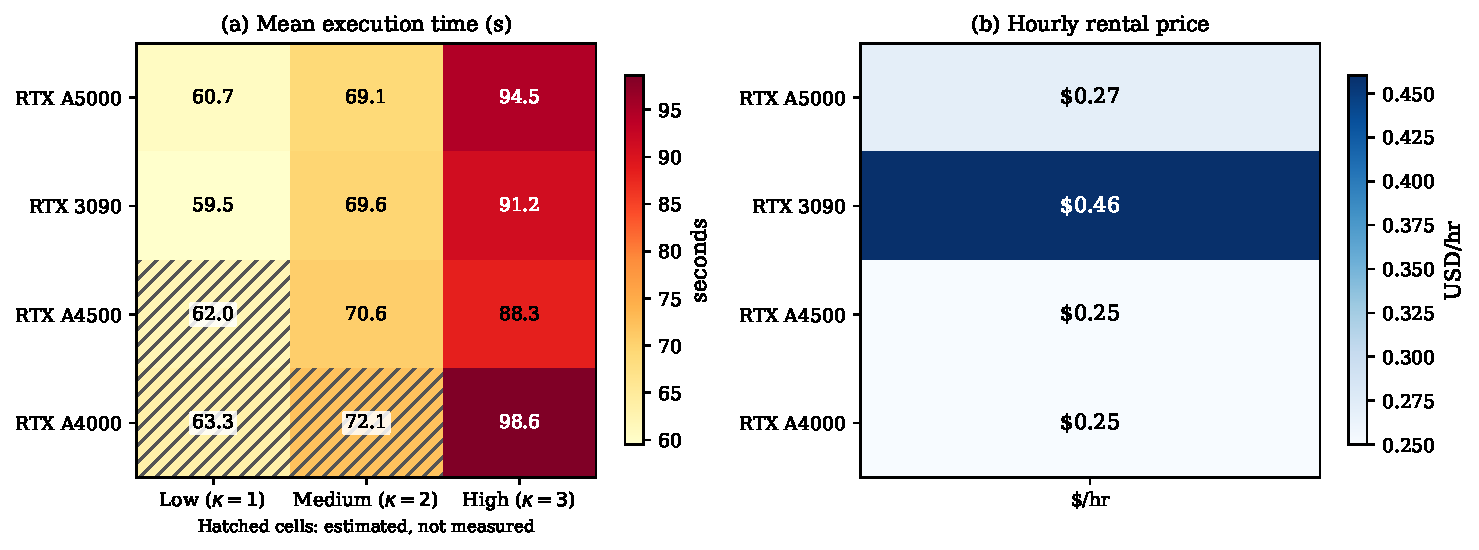
\includegraphics[width=0.98\linewidth,height=0.72\textheight,keepaspectratio]{figures/gpu_heatmap.pdf}
\caption[GPU fleet execution-time heterogeneity and pricing]{GPU fleet heterogeneity. Panel~(a): mean execution time (seconds) per GPU type and scene complexity level $\kappa$; the three model-estimated cells (low-complexity A4500 and A4000, medium-complexity A4000) are marked. The RTX~A4500 is fastest at high complexity (88.3\,s) despite having fewer CUDA cores than the RTX~3090 (91.2\,s), illustrating that the GPU speed ranking is non-monotone with respect to hardware specifications. Panel~(b): hourly rental price. The RTX~3090 is the most expensive (\$0.46/hr) yet has the lowest unweighted mean over the three complexity levels (73.4\,s, against 73.6\,s for the A4500 and 74.8\,s for the A5000, with three estimated cells included) and is second only to the A4500 at high complexity among the dense strata; the A4500 and A4000 share the same price (\$0.25/hr) while differing in speed, making node selection a genuine multi-criteria optimisation.}
\label{fig:gpu-heatmap}
\end{figure}
\end{landscape}

\section{Summary}
\label{sec:summary}

Table~\ref{tab:related_comparison} summarises the positioning of CGRSP relative to closely related work. Among the studies surveyed, CGRSP combines all four features the table compares: (1) real-world calibrated GPU heterogeneity, (2) stochastic qualitative availability (marketplace-driven, observed only as coarse stock status), (3) explicit deadline constraints, and (4) statistical evaluation across multiple seeds, day types, and concurrency limits. The table covers the foundational and GPU-scheduling studies; the three nearest recent works discussed above (SkyNomad, REACH, BOA Constrictor) are contrasted in the text rather than tabulated, and none of them observes availability as a coarse stock status. The per-second billing model is a property of the platform being modelled, not a compared dimension.

\begin{table}[htbp]
\centering
\small
\caption[Positioning of CGRSP against related work]{Positioning of CGRSP against related scheduling studies}
\label{tab:related_comparison}
\begin{tabular}{lcccc}
\toprule
\textbf{Work} & \textbf{GPU Hetero.} & \textbf{Stoch.\ Avail.} & \textbf{Deadlines} & \textbf{Stat.\ Valid.} \\
\midrule
Braun et al.~\cite{braun2001comparison} & Synthetic & \texttimes & \texttimes & \texttimes \\
HEFT~\cite{topcuoglu2002heft}           & Synthetic       & \texttimes & \texttimes & \texttimes \\
Mao et al.~\cite{mao2016resource}       & \texttimes & \texttimes & \texttimes & \checkmark \\
Chen \& Chen~\cite{chen2023gpu}             & Yes       & \texttimes & \texttimes & Limited \\
Ye et al.~\cite{ye2024deep}           & Yes (survey) & \texttimes & Partial   & \texttimes \\
Narayanan et al.~\cite{narayanan2020gavel} (Gavel) & Yes & \texttimes & Partial & \checkmark \\
\textbf{CGRSP (this thesis)}            & \checkmark & \checkmark & \checkmark & \checkmark \\
\bottomrule
\end{tabular}
\end{table}

Beyond the four dimensions in Table~\ref{tab:related_comparison}, CGRSP is, to the best of the author's knowledge, the first scheduling study of marketplace cloud GPU rental applied specifically to \emph{batch 3D rendering workloads}. Compared to deep learning training, the dominant focus of GPU scheduling literature~\cite{ye2024deep,peng2018optimus,narayanan2020gavel}, rendering frames have three properties that shape the scheduling design. First, execution is \emph{short and non-preemptive}: individual frames complete in tens of seconds to a few minutes, making checkpoint-and-resume impractical and favouring simple online dispatch policies over the long-horizon optimisation that DL training schedulers can exploit. Second, \emph{complexity is observable at submission}: scene complexity level ($\kappa$) is treated as known when a job enters the queue (in deployment it would be classified from scene statistics such as polygon and light counts that are available before rendering; in the calibration dataset it is proxied by render-time terciles, Section~\ref{ssec:platform-and-data}), providing the execution-time estimate that SPT and SPT+Rescue rely on. Third, \emph{GPU performance is non-monotone across complexity levels}: for high-complexity frames ($\kappa=3$), the RTX~A4500 (7,168 CUDA cores, 88.3\,s) has a lower observational stratum mean than the RTX~3090 (10,496 cores, 91.2\,s; see Table~\ref{tab:gpu_specs}), while at medium complexity the A5000 (69.1\,s) edges the 3090 (69.6\,s); these are not scene-matched evidence (Section~\ref{sec:gpu-fleet-model}), but they illustrate why the model uses per-complexity stratum means rather than a fixed GPU speed ranking. These three rendering properties shape the CGRSP formulation and calibration methodology.
